\documentclass[10pt,conference]{IEEEtran}

% Conference class (no compsoc / compsocconf).
\IEEEoverridecommandlockouts
\usepackage{graphicx}
\usepackage{cite}
\usepackage{booktabs}
\usepackage{tabularx}
\usepackage{tikz}
\usetikzlibrary{arrows.meta,positioning,shapes.geometric,fit,calc}
\usepackage{amsmath}
\usepackage{xurl}
\usepackage[hidelinks]{hyperref}
\usepackage{balance}
% Tighten float gaps after full-width figures/tables (layout review).
\setlength{\textfloatsep}{8pt plus 2pt minus 2pt}
\setlength{\floatsep}{8pt plus 2pt minus 2pt}
\setlength{\intextsep}{8pt plus 2pt minus 2pt}
\setlength{\dbltextfloatsep}{8pt plus 2pt minus 4pt}
\setlength{\dblfloatsep}{8pt plus 2pt minus 4pt}

\begin{document}

\title{From Pilot toward Conditional Scale: A Stage-Gated AI4SE Path for Mid-to-Large Software Organizations%
\thanks{J.~Qiu is Principal AI4SE Consultant at Inspire Group (Ph.D., Software Engineering, Tongji University; 18+ years in software engineering, R\&D productivity, and enterprise architecture).
Q.~Yan is AI4SE Engineering Advisor at Inspire Group (M.S., Computer Science, Sichuan University; 10+ years in enterprise architecture, DevOps, and AI-agent engineering).
Inspire Group is a technology-services firm formed from the former Thoughtworks China business after its acquisition by Hillhouse Capital (announced 2025); the Inspire authors facilitated the Org-A and Org-B engagements.
Industrial partners remain anonymized (Org-A, Org-B); no client co-authors.}}

% Inspire Group authors only; client declined co-authorship (2026-09 decision). Body keeps Org-A / Org-B anonymization + sector-type portraits.
\author{
\IEEEauthorblockN{Juan Qiu\IEEEauthorrefmark{1},
Qilong Yan\IEEEauthorrefmark{1}}
\IEEEauthorblockA{\IEEEauthorrefmark{1}Inspire Group, China\\
Emails: juan.qiu@inspiregroup.com,~qlyan@inspiregroup.com}
}

\maketitle

\begin{abstract}
Mid-to-large software organizations---multi-site engineering groups with enough
process inertia and cross-team handoff that a tool trial does not diffuse by
itself---often equate an AI-for-software-engineering (AI4SE) assistant rollout,
or a completed pilot increment, with readiness to scale.
As generation cost falls, scarce capacity shifts from coding throughput to
\emph{definition and verification}---knowing what is correct and proving it.
We report a stage-gated transformation path for that setting---Explore,
Consolidation, and conditional Scale---in which each gate is an evidence review
rather than a calendar event.
At Org-A, a six-week Explore engagement produced a citable method, countable
opportunity assets, and a readiness-labeled executable-asset ledger;
management passed the Explore gate and opened Consolidation, but did not
admit Scale.
As a secondary recognition observation, Org-B---a manufacturing enterprise
whose incumbent process is Integrated Product Development (IPD)---selected
the same path after co-located alternatives were judged infeasible and is now
in a mid-July to mid-September 2026 Explore that remains open.
The paper contributes the path and the Org-A gate-and-asset record; Org-B
supplies only a decision-fact vignette, not a second completed case.
It does not claim organization-wide scale, completed Scale admission, or
platform-measured return.
\end{abstract}

\begin{IEEEkeywords}
AI for software engineering, stage-gated transformation, industrial experience report
\end{IEEEkeywords}

\section{Introduction}
\label{sec:intro}
% EVIDENCE: ../outline.md §I; design spec §3

Sponsors of AI4SE programs face a recurring management error: equating access
to coding assistants, or completion of a facilitated pilot, with a
scale-ready organizational capability.
The first produces local tool use; the second may produce a one-off
demonstration.
Neither, by itself, answers whether a new team can run a complete cycle under
agreed guardrails.
Guidance on developer productivity already warns that a single activity or
throughput slogan is a poor decision aid~\cite{Forsgren2021SPACE}.
A sharper industrial reading is that AI coding assistance compresses
\emph{implementation} cost while amplifying errors that originate in vague
intent, weak specifications, and unverified agent output: the bottleneck
moves toward \emph{definition scarcity} and verification capacity.
The corresponding transformation error is to treat a well-received pilot as
authorization for organization-wide diffusion.

We report a stage-gated path for advancing industrial AI4SE without treating
calendar completion as admission---validated primarily by Org-A's real gate
disposition and asset ledger, not by a method brochure alone.
A stage has a purpose, work products, and an observable exit that is also an
admission test for the next stage.
Explore asks whether a method can be exercised end-to-end in a real delivery
context.
Consolidation asks whether the pilot team can repeat and teach that method.
Scale, entered only conditionally, asks whether a new team can complete a
cycle independently.
Org-A supplies the primary longitudinal evidence; Org-B supplies only a
bounded recognition vignette (local adoption after infeasible alternatives,
Explore still open).
The transferable object is the path-plus-gate contract---not a tool catalog
and not a completed rollout.

We organize the experience around three questions:
\begin{itemize}
\item \textbf{Q1.}
How can an industrial AI4SE path from pilot toward scale be designed
(goals, deliverables, and gate or exit tests)?
\item \textbf{Q2.}
What assets, signals, and admission boundaries did Org-A's completed Explore
produce in support of Consolidation and of only-conditional Scale?
\item \textbf{Q3.}
While Org-B is still in Explore, what does a local adoption decision after
infeasible alternatives show---and what does it not show?
\end{itemize}

\textbf{Methodological stance.}
This manuscript is an industrial experience report~\cite{Runeson2009CaseStudy}.
Facilitators co-designed the path with client teams, but the claims we defend
are those Org-A management actually gated (Explore pass / Scale hold) and the
readiness labels in the handoff ledger---practitioner-validated decisions,
not a consultant self-score.
Org-B remains a secondary recognition vignette~\cite{Hevner2004DSR}.
We do not claim multi-case theoretical saturation, a completed design-science
evaluate cycle, researcher-owned action-research agency, or completed Scale
at either organization.

\textbf{Contributions.}
(1)~a stage-gated AI4SE path with an admission contract (citable / runnable /
transferable readiness; stub~$\neq$~ready);
(2)~Org-A evidence that Explore completed, Consolidation started, and Scale
admission was not met---stated as a three-layer feasibility argument rather
than as assumed diffusion;
(3)~a bounded Org-B decision fact only: the same path was selected after
alternative approaches were judged infeasible, under an IPD constraint, with
Explore still open (not a second completed gate packet).

Bounded Explore-phase effectiveness and maturity signals appear here only as
gate inputs with stated limits.
A companion measurement manuscript (separate contribution; dual-lens labeled
reporting of capability and delivery signals at Org-A) owns how those signals
are stratified and later promoted from estimate to platform measurement; we
do not reproduce its tables or claim concurrent review of that companion
manuscript here.\footnote{Companion status at freeze: authoring for a
peer-reviewed software-engineering venue; unit of analysis $=$ measurement
scheme, not the stage-gated path.  No Org-A workshop or maturity numbers from
that manuscript are imported here.}

Section~\ref{sec:background} supplies the conceptual overlay.
Section~\ref{sec:path} defines the stages and gates.
Section~\ref{sec:org-a} reports Org-A.
Section~\ref{sec:org-b} reports Org-B.
Sections~\ref{sec:discussion}--\ref{sec:related-conclusion} discuss
takeaways, threats, related work, and the claim ceiling.

\section{Conceptual Background}
\label{sec:background}
% EVIDENCE: ../outline.md §II; design spec §1\#3 and §3.4 (AIDD as conceptual layer)
% Added 2026-08-30: Cynefin domain fit; Pressman layer inheritance; harness certainty boundary (adapted from Fowler)
% Added 2026-08-30: Thoughtworks Utah + Europe Future of Software Engineering retreat reports

The stage-gated path is the contribution of this paper.
This section supplies a compact vocabulary for \emph{why the path is staged}
and \emph{what it carries}.
It is not a second framework to be evaluated on its own, and it is not a
restatement of a practitioner slide deck.

\subsection{Domain Fit: Why Exploration Is Not Instant Scale}
\label{sec:cynefin}

Snowden and Boone's Cynefin framing distinguishes decision domains in which
best practice, expert analysis, or probe-and-sense behavior is
appropriate~\cite{Snowden2007Cynefin}.
Early industrial AI4SE work is typically \emph{complex}: workable method is
emergent, so Explore is a probe that must produce inspectable method assets
rather than a purchased best-practice pack.
Consolidation moves durable findings toward the \emph{complicated} domain:
playbooks, harness hardening, and seed coaches support sense--analyze--respond
transfer.
Scale entry is admitted only when enough of the method is stable to diffuse
without re-running full discovery---closer to clear or well-analyzed
complicated work, never by calendar alone.
The gates are therefore domain-fit devices: treating a Complex probe as Clear
rollout is the failure mode this paper records as ``pilot success without
Scale admission.''

\subsection{Industry Fault Lines as Staging Rationale}
\label{sec:tw-retreats}

Senior-practitioner syntheses from Thoughtworks' Utah and Europe Future of
Software Engineering retreats highlight fault lines that motivate
staging~\cite{Thoughtworks2026UtahRetreat,Thoughtworks2026EuropeRetreat}:
engineering rigor migrating into specifications, tests, and constraints; a
supervisory \emph{middle loop} between coding and delivery; verification
(not generation) as scarce capacity; harness ownership around the agent; and
a two-clock mismatch in which code-production time collapses while decision
time does not.
We use that map only as industrial \emph{rationale}.
Explore must freeze probe evidence; Consolidation must harden verification,
harness ownership, and seed coaches; Scale is admitted only when decision and
verification capacity can absorb a receiving team.
Retreat anecdotes are not Org-A/Org-B facts, and retreat consensus is not
empirical validation of our gates; denser positioning appears in
Section~\ref{sec:related-conclusion}.

\subsection{Layer Inheritance: Pressman Structure, Upgraded Semantics}
\label{sec:pressman}

Classical software-engineering textbooks present a layered view in which a
quality focus grounds process, methods, and tools, and in which more visible
layers depend on less visible ones~\cite{Pressman2014SEPA}.
Figure~\ref{fig:pressman-ai4se} states our industrial reading: the
\emph{structure} is inherited; the \emph{semantics} must be upgraded for
human--agent delivery.
Quality focus becomes \emph{Effectiveness} (quality plus waste-aware
efficiency).
Process, methods, and tools retain their roles, but executors are humans
\emph{and} agents.
Harness Engineering, Spec-Driven Development (SDD), and Agentic Engineering
are placed in the \emph{methods} family (discipline and assets), not as a
replacement for the process layer or as a tools-only purchase.
\emph{Harmony} is a cross-cutting human--agent contract, not a fifth stacked
layer.

\begin{figure}[t]
\centering
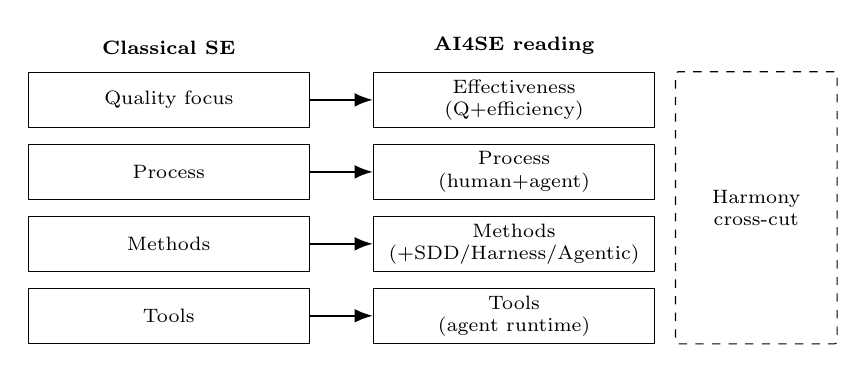
\begin{tikzpicture}[
  font=\scriptsize,
  box/.style={draw, align=center, inner sep=2.5pt, minimum height=7mm},
  layer/.style={box, text width=0.28\columnwidth},
  arr/.style={-{Latex}, thick}
]
\node[layer] (tq) {Quality focus};
\node[layer, below=2mm of tq] (tp) {Process};
\node[layer, below=2mm of tp] (tm) {Methods};
\node[layer, below=2mm of tm] (tt) {Tools};
\node[layer, right=8mm of tq] (aq) {Effectiveness\\(Q+efficiency)};
\node[layer, below=2mm of aq] (ap) {Process\\(human+agent)};
\node[layer, below=2mm of ap] (am) {Methods\\(+SDD/Harness/Agentic)};
\node[layer, below=2mm of am] (at) {Tools\\(agent runtime)};
% Harmony spans the full AI4SE stack height (Effectiveness .. Tools).
\path let \p1=(aq.north), \p2=(at.south), \n1={\y1-\y2} in
  node[
    draw, dashed, rounded corners=1pt,
    align=center,
    text width=0.15\columnwidth,
    minimum height=\n1,
    anchor=west
  ] (hh) at ($(aq.east)!0.5!(at.east)+(2.5mm,0)$)
    {Harmony\\cross-cut};
\draw[arr] (tq) -- (aq);
\draw[arr] (tp) -- (ap);
\draw[arr] (tm) -- (am);
\draw[arr] (tt) -- (at);
\node[above=1mm of tq, font=\scriptsize\bfseries] {Classical SE};
\node[above=1mm of aq, font=\scriptsize\bfseries] {AI4SE reading};
\end{tikzpicture}
\caption{Inherited layered software-engineering structure with upgraded
AI4SE semantics (conceptual).
Harness/SDD/Agentic sit primarily in Methods; Harmony cross-cuts rather than
stacking a fifth layer.}
\label{fig:pressman-ai4se}
\end{figure}

\subsection{Effectiveness, Harmony, and Four In-Path Directions}

We use two cross-cutting concerns---\emph{Effectiveness} and
\emph{Harmony}---and four capability directions: SDD, Agentic Engineering,
Harness Engineering, and an AI4SE Operating Model.
Figure~\ref{fig:aidd-on-path} maps them onto the stages of
Section~\ref{sec:path}.
We do not treat these labels as a maturity model, a vendor stack, or a
substitute for the gates.

\begin{figure}[t]
\centering
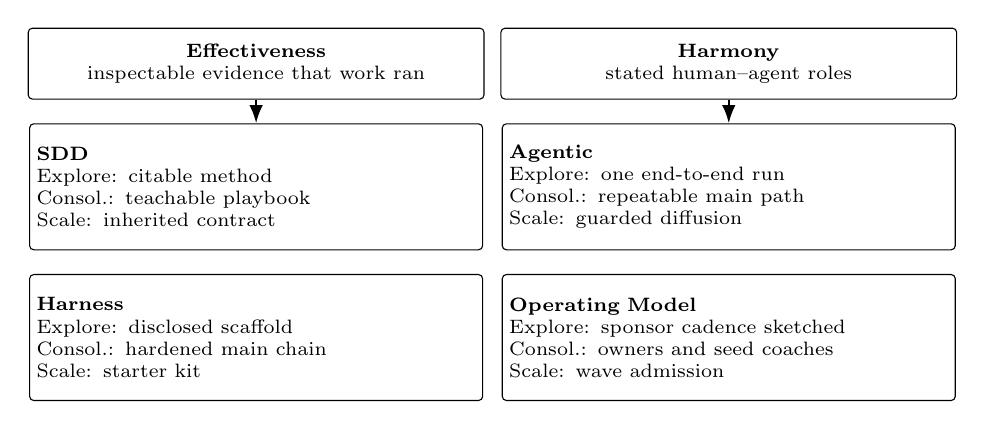
\begin{tikzpicture}[
  font=\scriptsize,
  >=Latex,
  concern/.style={
    draw,
    rounded corners=1.5pt,
    align=center,
    inner sep=3pt,
    text width=0.46\columnwidth,
    minimum height=9mm
  },
  dir/.style={
    draw,
    rounded corners=1.5pt,
    align=left,
    inner sep=2.5pt,
    text width=0.46\columnwidth,
    minimum height=16mm
  }
]
\node[concern] (eff) {\textbf{Effectiveness}\\inspectable evidence that work ran};
\node[concern,right=2mm of eff] (har) {\textbf{Harmony}\\stated human--agent roles};
\node[dir,below=3mm of eff] (sdd) {\textbf{SDD}\\Explore: citable method\\Consol.: teachable playbook\\Scale: inherited contract};
\node[dir,below=3mm of har] (ag) {\textbf{Agentic}\\Explore: one end-to-end run\\Consol.: repeatable main path\\Scale: guarded diffusion};
\node[dir,below=3mm of sdd] (hn) {\textbf{Harness}\\Explore: disclosed scaffold\\Consol.: hardened main chain\\Scale: starter kit};
\node[dir,below=3mm of ag] (om) {\textbf{Operating Model}\\Explore: sponsor cadence sketched\\Consol.: owners and seed coaches\\Scale: wave admission};
\draw[->,thick] (eff) -- (sdd);
\draw[->,thick] (har) -- (ag);
\end{tikzpicture}
\caption{Effectiveness, Harmony, and four capability directions mapped onto
the stage-gated path.
The overlay is conceptual; it is not a second evaluated contribution.}
\label{fig:aidd-on-path}
\end{figure}

Effectiveness is the requirement that each stage produce inspectable evidence
that the selected work actually ran under local constraints---a citable
method, a validation-vehicle run-through, or a new-team cycle---rather than
attendance counts or tool-license counts.
Harmony is the requirement that human and agent accountability be
\emph{operationalized}, not merely named.
In the engagements we distinguish four complementary functions that may be
held by fewer people in a small team but must not be vacant:
\emph{intent ownership} (what to build and what success means),
\emph{specification stewardship} (living specs and change deltas as the
shared source of truth),
\emph{AI-asset orchestration} (skills, recipes, and harness units that make
the method executable), and
\emph{verification leadership} (acceptance and gate sign-off).
A working rule is \emph{contract separation}: the party that proposes or
applies a change must not be the sole party that verifies it---agents may
draft and execute, but humans retain intent and verification authority.
Both Effectiveness and Harmony are inputs to G1 and G2.
They are not outcome multipliers, and this paper does not report them as
measured organizational return.

The four directions are stage-relative obligations.

\textbf{SDD} converts intent into specifications that agents and humans can
execute, review, and accept.
Explore must produce a first citable method; Consolidation must make that
method teachable; Scale uses it as the contract a receiving team inherits.
Spec-driven development paired with agentic execution is an active industrial
theme; Gupta discusses the pairing in a preprint on high-accuracy agentic
frameworks~\cite{Gupta2026SDDAgentic}.
We cite that work as thematic context, not as an evaluation of Org-A or
Org-B.

\textbf{Agentic Engineering} turns those specifications into composable,
reviewable agent work---skills, commands, and recipes---rather than ad-hoc
prompting.
Explore needs one end-to-end agentic run; Consolidation needs the principal
path to be repeatable by the pilot team; Scale admits that path only with
declared guardrails.

\textbf{Harness Engineering} is the runtime---context, tools, permissions,
feedback, and audit---in which agents operate.
Explore may leave the harness as a disclosed scaffold; Consolidation must
harden the main chain; Scale requires a starter kit another team can run.
A stub is not a production harness; Section~\ref{sec:org-a} operationalizes
that distinction in the Org-A ledger.

\textbf{Operating Model} covers owners, coaching, sponsor cadence, and wave
admission---including named holders of the Harmony functions above.
It is sketched in Explore, staffed in Consolidation (named owners and seed
coaches), and enforced at Scale entry.
Without it, a hardened harness still has no authorized receiving team.

\subsection{Certainty Boundary: User Harness, Model, and Method Assets}
\label{sec:harness-boundary}

Industrial harness writing emphasizes bounded contexts among users, coding
agents, and models~\cite{Fowler2026Harness}.
Figure~\ref{fig:harness-certainty} is our AI4SE reading of that idea for
transformation work: organizational certainty does not live in the model
alone.
We write the staged enablement object as a paradigm-conditioned composition
\begin{equation}
\mathcal{H}^{p}(x)
=
\mathrm{UserHarness}^{p}\!\big(
\mathrm{CodingAgent}^{p}\!\big(
\mathrm{Model}(x)
\big)
\big),
\label{eq:harness-compose}
\end{equation}
where \(p\) is the governing delivery paradigm (for example
spec-driven development versus loosely guided ``vibe coding,'' or an agile
variant).
The inner \(\mathrm{Model}\) is comparatively stable across engagements;
the outer two layers are where Explore must freeze inspectable structure and
Consolidation must harden ownership.
The same model under different \(p\) therefore yields different
\(\mathcal{H}^{p}\): an SDD-oriented user harness privileges contracts,
acceptance checks, and reviewable agent recipes, whereas a vibe-oriented
harness privileges fast prompt--edit loops and lighter formal gates.
Neither is universally ``correct''; the gate packet must record which \(p\)
was chosen and what evidence that choice requires.

Operationally, each outer layer is itself a composition of smaller units
around a frozen model operator \(M\):
\begin{equation}
\mathcal{H}_{\mathrm{single}}(x)
=
h_{k}\!\big(\cdots h_{1}\big(M(h_{0}(x))\big)\cdots\big),
\label{eq:harness-layers}
\end{equation}
with \(h_{0}\) assembling context and guides, \(h_{1}\) parsing and schema
checks, and later \(h_{i}\) covering tools, permissions, sensors, and
feedback.
\emph{Agentic engineering} is not a fourth paradigm competing with SDD or
vibe coding; it is the engineering style that turns a chosen \(p\) into
composable, executable, and verifiable AI assets---skills, subagents,
commands, rules, and hooks---inside \(\mathrm{UserHarness}^{p}\) and
\(\mathrm{CodingAgent}^{p}\).
Method assets (playbooks, SDD contracts, starter kits) feed those outer
layers; they do not replace the model.
The harness must remain an open class across SDD stacks (for example
OpenSpec-, Superpowers-, or Spec-Kit-style frameworks, and future peers),
not a lock-in to one template---a constraint Org-B makes explicit in
Section~\ref{sec:org-b}.

\begin{figure}[t]
\centering
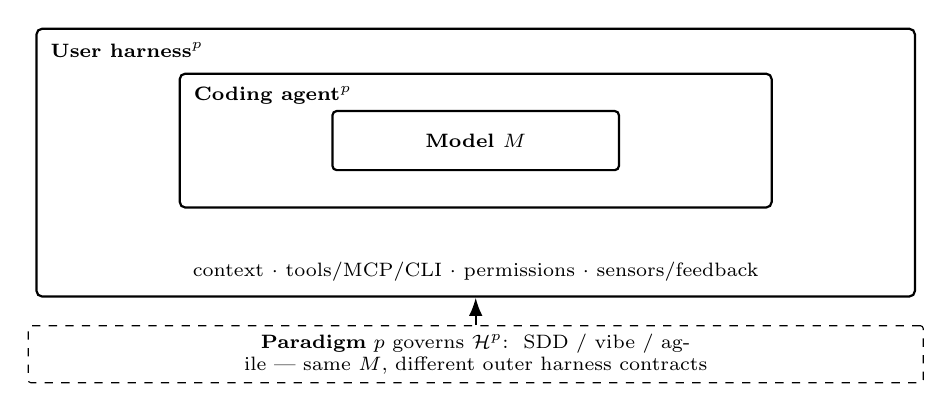
\begin{tikzpicture}[
  font=\scriptsize,
  >=Latex
]
% Top: nested certainty layers (full width; no side callout)
\node[
  draw, thick, rounded corners=2pt,
  minimum width=0.92\columnwidth, minimum height=34mm,
  align=center, fill=white
] (user) {};
\node[anchor=north west, font=\scriptsize\bfseries]
  at ([xshift=2pt,yshift=-2pt]user.north west) {User harness\(^{p}\)};
\node[anchor=south, align=center, font=\scriptsize]
  at ([yshift=2.5pt]user.south)
  {context $\cdot$ tools/MCP/CLI $\cdot$ permissions $\cdot$ sensors/feedback};

\node[
  draw, thick, rounded corners=2pt,
  minimum width=0.62\columnwidth, minimum height=17mm,
  align=center, fill=white
] (agent) at ([yshift=2.8mm]user.center) {};
\node[anchor=north west, font=\scriptsize\bfseries]
  at ([xshift=2pt,yshift=-1.5pt]agent.north west) {Coding agent\(^{p}\)};

\node[
  draw, thick, rounded corners=1.5pt,
  minimum width=0.30\columnwidth, minimum height=7.5mm,
  align=center, fill=white, font=\scriptsize\bfseries
] (model) at (agent.center) {Model \(M\)};

% Bottom: paradigm $p$ (replaces former method-assets strip)
\node[
  draw, dashed, rounded corners=1pt,
  align=center, inner sep=3pt,
  text width=0.92\columnwidth,
  below=3.5mm of user
] (paradigm) {%
  \textbf{Paradigm \(p\)} governs \(\mathcal{H}^{p}\):\,
  SDD / vibe / agile --- same \(M\), different outer harness contracts};
\draw[->,thick] (paradigm) -- (user.south);
\end{tikzpicture}
\caption{Certainty boundary for AI4SE enablement (conceptual adaptation of
harness bounded-context thinking~\cite{Fowler2026Harness}).
Top: nested layers realizing~(\ref{eq:harness-compose}).
Bottom: paradigm \(p\) selects the outer contracts
(Eq.~(\ref{eq:harness-layers})); method assets feed those outer units.
Agentic engineering composes them---it is not a competing fourth paradigm.}
\label{fig:harness-certainty}
\end{figure}

Skipping Consolidation typically leaves SDD prose and a stubbed harness in
the hands of a new team---the failure mode Section~\ref{sec:path} names as
equating a pilot with scale.
The conceptual layer therefore explains \emph{why} the gates ask for method,
asset, ownership, and transfer evidence; it does not add a parallel
transformation method.

\section{Stage-Gated Path}
\label{sec:path}
% EVIDENCE: ../00-shared-evidence/scale-path.md, phase1-gate.md

\subsection{Why a Gate, Rather Than a Calendar, Advances the Path}

We define an AI4SE transformation path as a sequence of capability-building
stages separated by explicit management decisions.  A stage has a purpose,
work products, and an observable exit condition.  Its exit condition is also
an admission test for the next stage: elapsed time can trigger a review, but
cannot substitute for evidence.  This distinction is important because a
pilot can finish on schedule while leaving its method tacit, its automation
fragile, or its ownership unresolved.
Collapsing code-production time does not by itself collapse decision and
verification time---another reason gates must review evidence rather than
calendars.

The transformation path nests two control loops.
\emph{Stage gates} (G1/G2) decide whether the organization may enter
Consolidation or admit a Scale wave.
Inside delivery work, shorter \emph{change gates}---align a delta
specification, verify a candidate increment, then merge and
archive---protect each change under the chosen paradigm \(p\).
Stage gates ask whether method, assets, and ownership are transferable;
change gates ask whether a particular change is definition-complete and
evidence-backed.
Confusing the two is a common failure: a team that passes local change
reviews can still fail G2 if receiving teams cannot inherit the method.

% FACT-III-A
The path instantiated at Org-A comprises \emph{Explore},
\emph{Consolidation}, and \emph{Scale} (Fig.~\ref{fig:stage-gates}).
Explore asks whether the method can be exercised end-to-end in a real
delivery context.  Consolidation asks whether the resulting method can be
repeated and taught by the pilot team.  Scale, which is entered only
conditionally, asks whether a new team can run a complete cycle
independently while retaining agreed guardrails.  Outputs therefore flow
forward as dependencies: the first-generation playbook and pilot assets feed
hardening; the hardened method, executable starter kit, role owners, and seed
coaches then support controlled diffusion.

\begin{figure*}[t]
\centering
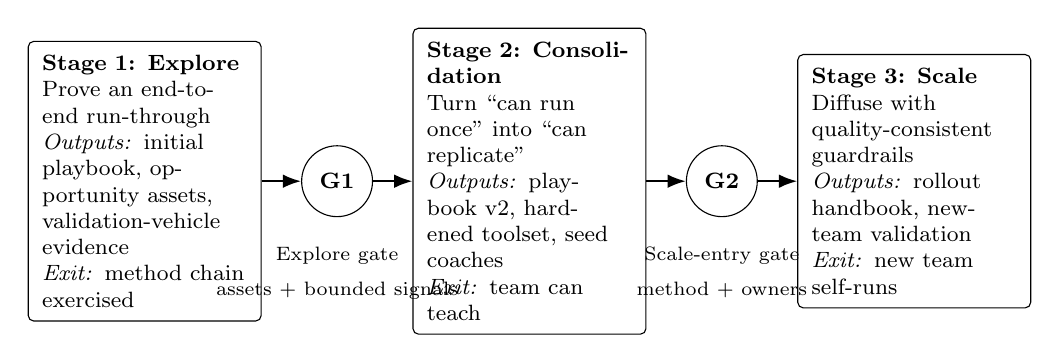
\begin{tikzpicture}[
  font=\footnotesize,
  >=Latex,
  stage/.style={
    draw,
    rounded corners=2pt,
    align=left,
    text width=0.215\textwidth,
    minimum height=24mm,
    inner sep=5pt
  },
  gate/.style={
    draw,
    circle,
    align=center,
    minimum size=9mm,
    inner sep=1pt,
    font=\footnotesize\bfseries
  },
  flow/.style={->,thick}
]
\node[stage] (explore) {
  \textbf{Stage 1: Explore}\\
  Prove an end-to-end run-through\\
  \emph{Outputs:} initial playbook, opportunity assets, validation-vehicle evidence\\
  \emph{Exit:} method chain exercised
};
\node[gate,right=5mm of explore] (g1) {G1};
\node[stage,right=5mm of g1] (consolidate) {
  \textbf{Stage 2: Consolidation}\\
  Turn ``can run once'' into ``can replicate''\\
  \emph{Outputs:} playbook v2, hardened toolset, seed coaches\\
  \emph{Exit:} team can teach
};
\node[gate,right=5mm of consolidate] (g2) {G2};
\node[stage,right=5mm of g2] (scale) {
  \textbf{Stage 3: Scale}\\
  Diffuse with quality-consistent guardrails\\
  \emph{Outputs:} rollout handbook, new-team validation\\
  \emph{Exit:} new team self-runs
};
\draw[flow] (explore) -- (g1);
\draw[flow] (g1) -- (consolidate);
\draw[flow] (consolidate) -- (g2);
\draw[flow] (g2) -- (scale);
\node[below=2.5mm of g1,align=center,font=\scriptsize] {Explore gate};
\node[below=7mm of g1,align=center,font=\scriptsize] {assets + bounded signals};
\node[below=2.5mm of g2,align=center,font=\scriptsize] {Scale-entry gate};
\node[below=7mm of g2,align=center,font=\scriptsize] {method + owners};
\end{tikzpicture}
\caption{Stage-gated AI4SE transformation path.  The figure specifies
evidence required to advance; it does not indicate that Org-A completed
Scale.}
\label{fig:stage-gates}
\end{figure*}

\subsection{Stages, Deliverables, and Exit Criteria}

% FACT-III-B
\textbf{Stage 1---Explore.}
The purpose of Explore is feasibility, not broad deployment.  In the Org-A
instantiation, the indicative duration was approximately six weeks, spanning
diagnosis and scenario selection, four workshop weeks over twelve opportunity
themes, co-creation of an initial playbook and executable-asset scaffold, and
use of a pilot change request as a validation vehicle.  The exit criterion
was an end-to-end run-through of the method chain.  It was deliberately not
completion of every feature in the validation vehicle.

% FACT-III-C
\textbf{Stage 2---Consolidation.}
Consolidation is the bridge between one successful run and a transferable
organizational capability.  Its indicative Org-A window was one to two
months.  The work comprises revising clauses that read correctly but do not
run in practice, hardening the principal executable path from stubs to usable
assets, assigning role ownership, and rehearsing coach-the-coach transfer.
Its intended products are a standardized playbook v2, a hardened toolset, and
seed coaches.
Hardening follows two practical rules drawn from the enablement practice:
\emph{do not promote immature automation} (skills and recipes must stabilize
before they are wrapped as autonomous agents), and \emph{keep apply separate
from verify} (an execution agent must not also issue the verification
verdict).
The exit condition is ``team can teach'': pilot-team members can explain and
transfer the method, rather than only reproduce a consultant-led
demonstration.

% FACT-III-D
\textbf{Stage 3---Scale.}
Scale is quality-consistent, wave-based diffusion rather than simultaneous
organization-wide rollout.  Admission requires the Consolidation exit,
named role owners, a starter kit for sibling teams, and reserved sponsor
cadence and resources.  Seed coaches then enable successive teams and review
practice consistency.  The terminal evidence is a fresh team's independent
completion of a cycle under the guardrails.  Thus, a calendar target can
prompt a G2 review, but an unmet G2 blocks admission.

\begin{table*}[t]
\caption{Decision tests at the two stage boundaries}
\label{tab:gate-tests}
\centering
\footnotesize
\begin{tabularx}{\textwidth}{@{}p{0.12\textwidth}X X X@{}}
\toprule
\textbf{Boundary} & \textbf{Evidence reviewed} &
\textbf{Positive decision} & \textbf{What the decision does not imply} \\
\midrule
G1: Explore closeout &
Citable playbook with gaps stated; inventory of converged and observed
opportunity assets; readiness of executable assets stated as ready or stub;
bounded effectiveness/maturity signals; discussable next-stage path &
The method chain ran end-to-end and the organization may enter
Consolidation &
All validation-vehicle features are complete; executable assets are ready
for broad use; measured organization-wide return has been established \\
\addlinespace
G2: Scale entry &
Team-can-teach evidence; hardened main execution path; named role owners;
starter kit; sponsor rhythm and resources &
A controlled wave may admit a new team with seed-coach support &
The Explore pilot alone authorizes diffusion; every team is already
independent; rollout outcomes are known in advance \\
\bottomrule
\end{tabularx}
\end{table*}

\subsection{Gate Semantics}

% FACT-III-E
G1 is a \emph{method--asset gate}.  Management asks whether a playbook can be
shown and cited with its gaps visible; whether opportunity-point
specifications and best practices can be inventoried; whether executable
assets are distinguished as ready or stub; whether effectiveness
and maturity signals carry their measurement boundaries; and whether the
Consolidation-to-Scale path is concrete enough to discuss.  A positive G1
therefore licenses method hardening, not broad rollout.  Table
\ref{tab:gate-tests} makes this decision contract explicit.

G2 is stricter because it concerns transfer beyond the pilot setting.  It
tests whether know-how has moved from individuals into teachable guidance,
executable assets, role ownership, and an enablement mechanism---and whether
verification authority remains human-held under the nested change gates.
The resulting admission decision is reversible and wave-specific: if a new
team cannot operate with the starter kit and bounded coaching, the
organization returns the deficient asset or role arrangement to
Consolidation.
This interpretation makes a gate a learning control, rather than a ceremonial
approval checkpoint.

\subsection{Operating a Gate as an Evidence Review}

A usable gate needs a review packet, a decision owner, and a recorded
disposition.  The review packet should present the stage goal first and then
map each promised output to an inspectable artifact or observation.  A
readiness label accompanies each item so that ``exists,'' ``runs on the
primary path,'' and ``transferable to a new team'' cannot collapse into one
category.  Known gaps remain in the packet as decision inputs.  Removing
them from view would make an approval easier to obtain but less useful for
planning the next stage.

The decision owner evaluates sufficiency for the \emph{next} stage, not
perfection in the current one.  At G1, an incomplete executable scaffold can
be acceptable when it is disclosed and when the Consolidation plan names the
hardening work.  At G2, the same scaffold is a blocker because a receiving
team would depend on it.  This relative interpretation prevents two common
errors: rejecting useful Explore evidence because every asset is not yet
finished, and admitting Scale because unfinished assets were tolerated at
Explore closeout.

A gate disposition has three possible forms.  \emph{Advance} means the exit
condition is met and the next stage may start under its declared scope.
\emph{Advance with conditions} records a narrow action whose completion is
checked before a dependent activity begins; it must not be used to waive a
core exit condition.  \emph{Hold} returns named gaps to the current stage.
In all three forms, the evidence and rationale remain available for the next
review.  This creates continuity across decisions and makes negative
evidence---for example, a stubbed primary path or missing owner---actionable
rather than embarrassing.

The gate also separates two kinds of uncertainty.  Product uncertainty asks
whether AI4SE can improve the selected work under local constraints; Explore
reduces it through actual method use.  Transfer uncertainty asks whether
another team can reproduce that use without recreating the method; only
Consolidation and a new-team test can reduce it.  Treating these uncertainties
separately explains why a positive G1 and a negative G2 can be the expected,
internally consistent outcome of the same review.

\subsection{Three-Layer Scale-Feasibility Argument}

The path permits a useful feasibility judgment before claiming completed
diffusion.  We structure that judgment in three layers.

\textbf{Layer 1---the path is designed.}
Goals, work products, exits, and admissions are stated before scale readiness
is assessed.  This makes the claim falsifiable: missing ownership, hardening,
or transfer evidence can stop advancement even when a pilot was well
received.

% FACT-III-F
\textbf{Layer 2---Explore is validated end-to-end.}
For Org-A, the initial playbook, opportunity assets, and validation vehicle
exercised the method chain under real delivery constraints.  The evidence
supports ``can run once'' and justified passing G1; it does not establish
repeatability across teams.

% FACT-III-G
\textbf{Layer 3---Scale remains conditional.}
Org-A's pilot succeeded at Explore, but G2 was not met at closeout.
Consolidation---including asset hardening and team self-solve
capability---is the prerequisite for a later Scale decision.  The feasibility
judgment therefore rests on an explicit path, observed end-to-end use, a
readiness-labeled asset ledger, and testable admission conditions.  It does
not rest on an assumed organization-wide return or on diffusion that has not
occurred.

\subsection{Anti-Patterns Exposed by the Gates}

\textbf{Tool-only transformation} treats access to a coding assistant or
plugin catalog as the change itself.  It omits the specifications,
verification, context, roles, and learning routines needed to make tool use
repeatable.  G1 exposes this weakness by requiring a citable method and
bounded evidence; G2 exposes it by requiring transfer and ownership.

\textbf{Pilot equals scale} converts a successful demonstration directly
into rollout authorization.  It conflates end-to-end feasibility with
cross-team replicability.  Separating G1 from G2 preserves the useful result
of the pilot while making the missing admission evidence visible.

\textbf{Skipping Consolidation} carries first-generation prose and stubs
directly into new teams.  The likely burden then moves from explicit
hardening to repeated local improvisation.  The Stage-2 exit---team can
teach---requires the organization to remove that burden before opening a
Scale wave.

\textbf{Agent self-certification} lets the same generative path that applied
a change also declare the change verified.  Nested change gates and the
Harmony verification function exist to forbid that shortcut: drafts and
execution may be agentic; gate sign-off remains human.

\section{Case Org-A}
\label{sec:org-a}
% EVIDENCE: ../00-shared-evidence/timeline.md, asset-ledger-L1-L4.md, consolidation-signals.md

\subsection{Industrial Context and Evidence Basis}

% FACT-IV-A
Org-A is an anonymized large global container-shipping and logistics
enterprise with a substantial, multi-site in-house IT organization
supporting commercial and operational systems.  The engagement was an
approximately six-week AI4SE enablement pilot, not a scale-out program.  The
delivery setting used a multi-team agile model, shared requirements
management, and distinct development, business-analysis, and quality roles.
Quality remained a standing constraint: efficiency exploration was not
allowed to relax the client's existing quality gates.

We report the case as an industrial experience and preserve a chain from each
case statement to a frozen evidence slice, following the traceability
principle in case-study reporting \cite{Runeson2009CaseStudy}.  The primary
case record comprises the phase timeline, the management gate definition,
the L1--L4 handoff ledger, and post-closeout consolidation signals.  We treat
the playbook and executable assets as designed artifacts evaluated through
use in their organizational environment, consistent with design-science
evaluation logic \cite{Hevner2004DSR}.  This paper uses only qualitative
signal boundaries from the evidence pack; measurement results are reserved
for the companion measurement study.

\subsection{Explore Activities}

\begin{figure*}[t]
\centering
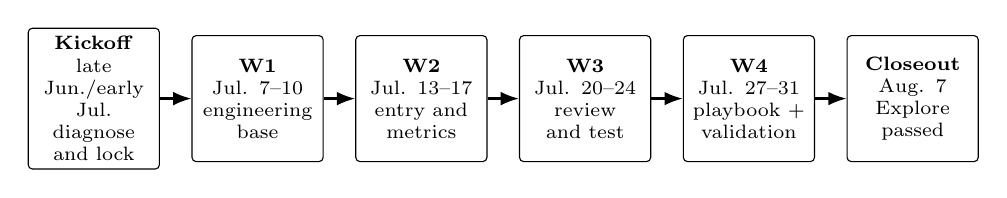
\begin{tikzpicture}[
  font=\scriptsize,
  >=Latex,
  event/.style={
    draw,
    rounded corners=1.5pt,
    align=center,
    text width=0.12\textwidth,
    minimum height=16mm,
    inner sep=3pt
  },
  flow/.style={->,thick}
]
\node[event] (kickoff) {\textbf{Kickoff}\\late Jun./early Jul.\\diagnose and lock};
\node[event,right=4mm of kickoff] (w1) {\textbf{W1}\\Jul. 7--10\\engineering base};
\node[event,right=4mm of w1] (w2) {\textbf{W2}\\Jul. 13--17\\entry and metrics};
\node[event,right=4mm of w2] (w3) {\textbf{W3}\\Jul. 20--24\\review and test};
\node[event,right=4mm of w3] (w4) {\textbf{W4}\\Jul. 27--31\\playbook + validation};
\node[event,right=4mm of w4] (close) {\textbf{Closeout}\\Aug. 7\\Explore passed};
\draw[flow] (kickoff) -- (w1);
\draw[flow] (w1) -- (w2);
\draw[flow] (w2) -- (w3);
\draw[flow] (w3) -- (w4);
\draw[flow] (w4) -- (close);
\end{tikzpicture}
\caption{Org-A Explore timeline.  The August 7 closeout passed the Explore
gate and opened Consolidation; it did not pass Scale admission.}
\label{fig:org-a-timeline}
\end{figure*}

% FACT-IV-B
The Explore phase followed a six-block arc (Fig.~\ref{fig:org-a-timeline}).
Kickoff in late June or early
July 2026 established the diagnosis, scenario lock, baseline maturity
exercise, and opportunity-theme plan.  Workshop W1 (July 7--10) addressed
engineering foundations: harness/context, knowledge, and brownfield
specification-driven development.  W2 (July 13--17) covered metrics and
requirements entry and ended with a midterm management showcase.  W3 (July
20--24) addressed review, agent validation, and test engineering.  W4 (July
27--31) ran two tracks in parallel: playbook v0.5 authoring and
specification-based validation in the delivery track.  The executive readout
on August 7 closed Explore, aligned the Consolidation path, and explicitly
did not claim Scale admission.

% FACT-IV-C
Across those four workshop weeks, the team worked through twelve opportunity
themes and co-created initial method and opportunity assets.  A pilot change
request supplied the validation vehicle for using the method in delivery.
This choice kept acceptance focused on whether the chain from opportunity
through specification and practice could be exercised, rather than on
shipping all business scope.  The activity record consequently supports a
process-feasibility conclusion, not a claim about broad adoption.

\subsection{From Activities to Gate Evidence}

The workshop sequence was not treated as attendance evidence.  Each block
was expected to leave a trace in one or more asset layers.  Foundation work
informed the method guidance and executable scaffold; opportunity work
created specifications and best practices; delivery-track use tested whether
those descriptions could guide action; and the closeout evidence pack
recorded both observed signals and their limits.  This trace converted a
series of facilitated sessions into inspectable inputs to G1.

The parallel tracks in W4 were particularly important to that conversion.
Playbook authoring alone could have produced guidance that was internally
coherent but detached from delivery.  Delivery work alone could have
produced a one-off result whose method remained tacit.  Running authoring and
specification validation together created a feedback loop: delivery exposed
where wording or executable support was weak, while the playbook gave the
team a stable object to revise and later cite.  The gate then assessed the
resulting artifacts and disclosed gaps rather than inferring capability from
workshop completion.

We used three readiness distinctions when interpreting the handoff.
\emph{Citable} means an artifact is stable enough to identify and discuss.
\emph{Runnable} means that its principal path works in the intended local
workflow.  \emph{Transferable} adds the ability of another team to use that
path with declared guardrails and bounded coaching.  Explore required a
citable method and evidence of local use; Scale admission would require
runnable and transferable support.  The distinctions explain why the L1
playbook could satisfy its G1 criterion while the largely stubbed L3 pack
could not satisfy G2.

\subsection{L1--L4 Outcomes and Readiness}

The closeout inventory was organized into four layers (Table
\ref{tab:asset-readiness}).  The layers distinguish descriptive guidance,
reusable opportunity knowledge, executable support, and evidence.  More
importantly, the ledger records readiness separately from existence; a
catalog entry is not treated as a deployable capability.

\begin{table*}[t]
\caption{Org-A Explore asset ledger at closeout}
\label{tab:asset-readiness}
\centering
\footnotesize
\begin{tabularx}{\textwidth}{@{}p{0.06\textwidth}p{0.20\textwidth}X p{0.24\textwidth}@{}}
\toprule
\textbf{Layer} & \textbf{Asset class} & \textbf{Observed outcome} &
\textbf{Readiness boundary / Consolidation need} \\
\midrule
L1 & Method playbook / operations handbook &
Version 1.0 was frozen, citable, and sufficient for the Explore gate. &
It was not playbook v2; clauses that read well but do not run remained
targets for revision. \\
\addlinespace
L2 & Opportunity specifications and best practices &
The release index contained 11 best practices and 11 specifications;
opportunity themes \#5 and \#9 remained observation items. &
Countability did not mean that every theme had converged. \\
\addlinespace
L3 & Executable plugins, skills, and recipes &
The formal pack, including the \texttt{/sdd} path, skills, recipes, and
adapters, was catalogued but largely stubbed on the main chain. &
\textbf{A stub is not production-ready.}  Main-chain hardening was Stage-2
work. \\
\addlinespace
L4 & Maturity/effectiveness evidence pack &
The handoff included evidence pointers and signal-type boundaries. &
The signals were process observations and expert estimates, not
platform-measured return; this paper does not reuse their numeric results. \\
\bottomrule
\end{tabularx}
\end{table*}

% FACT-IV-D
\textbf{L1: citable method.}
The frozen v1.0 handbook captured the end-to-end method---including how
intent becomes living specifications, change deltas, and accepted
increments---well enough to be shown and referenced at the gate.
Its frozen state made the Explore result auditable; it did not mean that
Consolidation revisions were complete.
Playbook v2 remained a Stage-2 target.

% FACT-IV-E
\textbf{L2: countable opportunity knowledge.}
The release set indexed 11 best practices and 11 corresponding
specifications across twelve named themes:
AI-ready story/living specification; UI prototyping; AI artifact review;
cycle-time/AI-effectiveness measurement design; role handoff (observation);
user harness/context pack; knowledge-base grounding; test engineering;
token/model routing (observation); brownfield specification-driven
development; agent nondeterminism evaluation; and CI toward AI control-system
checks.
Themes \#5 and \#9 retained observation status rather than being presented as
fully converged, so management could count the handoff without erasing
uncertainty within it.

% FACT-IV-F
\textbf{L3: scaffold, not production readiness.}
The handoff contained a formal executable-asset pack whose redacted layout
was:
\texttt{commands/} (\texttt{/sdd} catalog),
\texttt{skills/\{intent,spec,design,verify,harness\}/},
\texttt{recipes/} (ordered stage sequences),
\texttt{adapters/} (coding-agent hosts), and
\texttt{agents/} (sample wrappers only).
The catalog existed, but the main execution chain was largely stubbed:
many skill bodies were scaffolds, and stage recipes were not yet a hardened
primary path.
Org-A therefore recorded the assets as present but did not infer production
readiness from the directory tree, and did not treat early agent wrappers as
mature automation.
Moving the primary chain from stub to ready was explicitly assigned to
Consolidation.

The validation vehicle was a pilot change request on a live delivery track:
the team exercised intent capture, living-specification update, increment
application, and human-owned verification under retained quality gates.
Acceptance for Explore stayed on whether that method chain could be run and
cited, not on shipping the vehicle's full business scope.
We do not report cycle-time or defect metrics for the vehicle here; those
belong to the companion measurement manuscript.

As an illustrative L1 extract (paraphrased, not a verbatim client clause):
v1.0 required that every accepted increment cite a living-specification delta
id, name a human verifier distinct from the apply agent, and refuse
``generated-output equals verified'' shortcuts.
Org-A's later Consolidation agenda explicitly included rewriting clauses that
``read right but did not run'' on the main L3 chain---a recurring failure mode
for early playbooks.
Non-ROI intensity at closeout was gate-visible without claiming return:
four workshop weeks plus kickoff/readout, twelve themes (ten released),
$11{+}11$ L2 assets, a largely stubbed L3 main chain, and G1~pass / G2~hold.


% FACT-IV-G
\textbf{L4: bounded evidence.}
The evidence layer contained maturity and effectiveness materials and stated
their signal types.  Workshop judgments were expert estimates and the
materials were not presented as platform-measured return.  For this path
paper, L4 establishes that evidence boundaries were available to the gate;
it is not used to introduce the companion paper's quantitative findings.

\subsection{Phase-One Gate Decision}

% FACT-IV-H
At the August 7 executive readout, management applied five questions: whether
the playbook was citable; whether opportunity assets were countable; whether
executable readiness was labeled ready or stub; whether effectiveness and
maturity signals carried boundaries; and whether the next-stage path could
be discussed concretely.  The result was a pass for the Explore gate.  The
method had run end-to-end, the initial playbook and countable opportunity
assets existed, and bounded signals could be reported.

% FACT-IV-I
The same review did \emph{not} pass Scale admission.  Replicability and seed
coaches had not yet been demonstrated, the principal L3 execution chain
remained largely stubbed, and the role, starter-kit, sponsor-cadence, and
resource prerequisites were not all in place.  This was not a contradictory
verdict.  G1 answered whether the organization had enough evidence to harden
a feasible method; G2 would answer whether that hardened method could be
transferred to another team.

The two-part decision is the practical value of the path.  Without distinct
gates, management would have had to label the pilot either a failure because
it was not ready for broad diffusion, or a scale success because it completed
its planned activities.  The stage-gated account preserves the observed
Explore achievement and the unresolved admission work at the same time.

\subsection{Consolidation Started; Scale Entry Remained Conditional}

% FACT-IV-J
After the August 7 closeout, Org-A entered Consolidation, with an indicative
one-to-two-month window from early August through the end of September 2026.
The active work was framed as upgrading playbook v1 toward a standardized
v2 and hardening the L3 main chain.  Seed coaches and ``everyone can teach''
were capability targets and the Stage-2 exit criterion; they were not
reported as achieved at Explore closeout.

% FACT-IV-K
A consulting-side training and certification design also described
Foundation, Practitioner, and Seed Coach tracks and a team-readiness
certification concept.  It was a cross-customer capability-preparation
artifact at design-specification status: courseware, item bank, and learning
platform implementation were pending.  It therefore corroborates that scale
enablement was being designed, but it is not evidence that Org-A executed
training waves.

% FACT-IV-L
The resulting case posture is bounded but operationally useful.  Layer 1 of
the feasibility argument was in place because stages and gates had been
defined.  Layer 2 was observed because Org-A completed an end-to-end Explore
cycle and passed G1.  Layer 3 remained conditional because G2 had not been
met: later Scale admission depended on the team-can-teach result, named
owners, a hardened starter kit, and sponsor support.  An indicative October
calendar horizon was subordinate to those conditions.  No new-team
self-run, wave rollout, or organization-wide adoption was evidenced at the
freeze point.

Org-A thus illustrates why movement from pilot evidence toward conditional
Scale is a managed transition rather than a retrospective relabeling of
pilot success.  The case supplies
evidence for feasibility, asset creation, and the start of hardening.  It
also supplies explicit negative evidence---stubs, missing transfer proof, and
unmet prerequisites---that prevented an unsupported Scale claim.  A later
assessment can apply G2 to those same declared conditions without changing
the meaning of the Explore result.

\section{Case Org-B}
\label{sec:org-b}
% EVIDENCE: ../00-shared-evidence/org-b-adoption.md

\subsection{Industrial Context and Evidence Basis}

% FACT-V-A
Org-B is an anonymized manufacturing enterprise.
Unlike Org-A's multi-team agile setting, Org-B's incumbent product-development
regime follows Integrated Product Development (IPD).
The AI4SE path must therefore be adapted to IPD decision and lifecycle
structure.
We do not report a clause-level mapping of G1 or G2 onto Org-B's IPD
decision points; that mapping is a design constraint for Explore, not an
observed process rewrite.
We do not claim that Org-B has completed an organization-wide IPD$\times$AI4SE
rewrite.

% FACT-V-B
The evidence basis is an author briefing aligned to the statement of work
(SOW).
There is no consultant-side workspace mirror: client work remains on the
client intranet.
Facts in this section are therefore SOW- and briefing-level, and we mark
delivery status explicitly.

\subsection{Adoption After Infeasible Alternatives}

% FACT-V-C
From about mid-July through mid-August 2026, other co-located consulting
approaches led early exploration.
Org-B concluded that those AI4SE transformation approaches were not feasible
for its setting and selected the stage-gated path described here as the
primary Explore method.
We report this as a client decision outcome.
We do not name the alternative providers, and we do not present a competitive
scorecard.

% FACT-V-D
From that transition through late August 2026, this team has been guiding
multiple pilot teams through product research-and-development process
analysis under the path.
The calendar Explore window is mid-July to mid-September 2026.
As of the manuscript freeze (late August 2026), Explore remains in progress.
We do not write Org-B as Explore-closed, Consolidation-complete, or
organization-wide scaled.

\subsection{Multi-Mode Pilots under an IPD Constraint}

% FACT-V-E
The Explore wave intentionally samples heterogeneous software modes rather
than a single representative team embedded software; internal-use application development; large, complex
enterprise business systems; and AI-agent-oriented development.
Mode diversity is a sampling design for this Explore wave, intended to
exercise heterogeneous delivery constraints inside one organization.
It is not a completed mode-by-mode outcome set, and it is not evidence of
enterprise rollout or of a multi-enterprise sample.

\subsection{Harness Intent, Scope, and Vignette Bound}

% FACT-V-F
The intended user-harness layer is SDD-oriented and non-exclusive: it should
interoperate with Spec-Driven Development stacks of the OpenSpec /
Superpowers / Spec Kit \emph{class} (illustrative, not an allow-list) and
remain extensible to peers, with MCP/CLI hooks into Org-B's internal toolchain.
We claim neither production-complete integration nor single-stack lock-in.

% FACT-V-G
The SOW mixes Explore work with later-stage preparation: Goals~1--2 (method /
harness toolkit and end-to-end playbook) are Explore targets still open at
freeze; Goals~3--4 (training/certification and seed coaches) are
scale-preparation items, not observed Consolidation/Scale outcomes; Goal~5
is measurement-scheme design only (no Org-B numbers here).

As a recognition vignette, Org-B shows only that an IPD manufacturer can
record a local feasibility decision and start a multi-mode Explore under
harness-portability constraints.
It does not show that alternatives failed in general, that Explore closed,
that deliverables were accepted, or that Consolidation or organization-wide
scale has started.
Concrete negative process evidence at freeze: G1/G2 host reviews inside IPD
are not yet mapped; that absence is an Explore design debt, not a completed
IPD$\times$AI4SE rewrite.

\section{Discussion}
\label{sec:discussion}

\subsection{Reading the Two Cases Together}

Org-A and Org-B occupy different positions on the same path
(Table~\ref{tab:a-b-contrast}), with unequal evidence depth.
Org-A is the primary case: Explore completed, Consolidation started, Scale
admission withheld, with an in-repo ledger and gate packet.
Org-B is a secondary recognition vignette: the path was selected after
alternatives failed a local feasibility test, and Explore remains open under
IPD.
The shared path vocabulary can be named in more than one process heritage;
that does not make Org-B a second completed case.

\begin{table}[t]
\caption{Org-A and Org-B on the same path}
\label{tab:a-b-contrast}
\centering
\footnotesize
\begin{tabularx}{\columnwidth}{@{}p{0.22\columnwidth}X X@{}}
\toprule
 & \textbf{Org-A} & \textbf{Org-B} \\
\midrule
Calendar & $\sim$6-week Explore finished; Consolidation started & $\sim$2-month Explore, mid-July--mid-September; in progress \\
Process & Multi-team agile; retained quality gates & IPD incumbent; path must adapt \\
Pilot shape & Enablement plus validation vehicle & Multi-mode team sample in one wave \\
Adoption & Sponsored enablement; G1 pass / G2 hold & Method switch after infeasible alternatives \\
Harness & Playbook and plugin pack in handoff; main chain stubbed & Extensible multi-SDD harness plus MCP/CLI; not locked to one stack \\
Evidence depth & In-repo ledger and gate packet & Author briefing; no intranet mirror \\
\bottomrule
\end{tabularx}
\end{table}

The contrast also clarifies what ``method recognition'' is allowed to mean.
Org-B's switch is a decision fact about local feasibility, not a proof that
the path dominates unnamed alternatives in general, and not a claim that
Org-B has already produced Org-A's L1--L4 ledger.
IPD remains a stated incumbent constraint: this paper does not exhibit
which IPD reviews will host G1 or G2 at Org-B, and it does not invent
mid-September Explore closeout status.

Generic Stage-Gate practice already separates phases with business-case
reviews~\cite{Cooper1990StageGate}.
The incremental experience recorded here is narrower: an AI4SE admission
contract that treats a stubbed executable chain as Consolidation work,
publishes a withheld Scale decision beside a passed Explore gate, and
treats a second organization's still-open Explore as recognition rather
than as a completed case.
We do not claim a new general stage-gate theory.

\subsection{Manager Takeaways (Actionable)}

\begin{enumerate}
\item \textbf{Next week (50+ engineer org).}
Pick one delivery stream; freeze paradigm \(p\) and harness
\(\mathcal{H}^{p}\) (for Org-A, SDD-oriented); ban tool-only rollouts that
skip a citable method and a readiness-labeled ledger.
\item \textbf{At the first executive readout.}
Put G1 and G2 on separate agenda lines.
Ask the five Explore questions (citable method; countable opportunity
assets; stub/ready labels; bounded signals; discussable Consolidation path)
before any Scale calendar is debated.
\item \textbf{Playbook v1 clauses that flip first (Org-A lesson).}
(i)~guidance that ``reads right'' but has no runnable L3 path;
(ii)~promoting stub skills into autonomous agents;
(iii)~letting the apply path self-certify verify.
Rewrite those before opening a second team.
\item \textbf{Before any Scale wave.}
Name intent/spec/orchestration/verification owners, designate seed coaches,
and ship a starter kit another team can run; keep unmet G2 items on a public
hold list.
\item \textbf{Keep negative evidence visible.}
An unmet Scale gate, an in-progress Explore, and unaccepted deliverables are
decision inputs---not narrative failures to hide.
\end{enumerate}

\subsection{Boundary with the Measurement Companion}

This paper uses bounded effectiveness and maturity materials only as
qualitative gate inputs (Org-A L4; Org-B Goal~5 as scheme design).
The companion measurement paper's unit of analysis is a dual-lens reporting
scheme---labeled capability and delivery signals at Org-A---not the
stage-gated path.
The two manuscripts share a short anonymized Org-A context and the same
enablement window; they do not share main figures, and we do not import
that paper's tables or treat its workshop or maturity numbers as results of
the path.

\section{Threats to Validity}
\label{sec:threats}
% EVIDENCE: ../00-shared-evidence/threats-to-validity.md (Paper B subsection)

\textbf{External validity.}
The primary longitudinal case is a single organization (Org-A).
Org-B is an in-progress Explore at manuscript freeze, not a balanced
second site with a matching gate packet.
Mode diversity inside Org-B improves within-organization coverage; it does
not create a multi-enterprise sample.

\textbf{Construct validity.}
``Scale-ready'' is a gate-and-asset construct in this paper, not a
platform-measured return construct.
Absence of completed rollout must not be read as proof that the method is
ineffective, and bounded Explore signals must not be read as Scale
completion.

\textbf{Internal validity / observer bias.}
Authors facilitated enablement, gate framing, and asset authoring at
Org-A, and they are guiding Org-B's Explore.
Consolidation and readiness judgments may reflect consultant--client
alignment rather than independent audit.
We mitigate by binding factual sentences to a frozen evidence pack, by
publishing negative evidence (stubbed L3; unmet G2; Org-B still in
Explore), and by recording gate dispositions as client management decisions
(Advance / Hold) rather than as consultant self-scores.

\textbf{Org-B verification limits.}
Org-B prose relies on an SOW-aligned author briefing.
The absence of an intranet artifact mirror limits external checking of
those claims.
The adoption-after-alternatives account is given at sector and pattern
level without naming providers, so readers cannot independently reconcile
competitive context.

\textbf{Conclusion validity.}
A positive G1 plus a negative G2 is an internally consistent pair, not a
contradictory evaluation.
Treating either gate as a completed-scale result, or treating Org-B's
in-progress Explore as a second completed case, would be an invalid
conclusion.

\section{Related Work and Conclusion}
\label{sec:related-conclusion}

\subsection{Related Work}

\textbf{Methodological positioning.}
We follow software-engineering case-study guidance on context, chain of
evidence, and threats~\cite{Runeson2009CaseStudy}, and we treat the
stage-gated path as a designed enablement artifact~\cite{Hevner2004DSR}
illustrated primarily at Org-A.
We do not claim theoretical saturation or a completed design-science
evaluate cycle with field-measured Scale outcomes.

\textbf{Productivity caution, not a measurement contribution.}
Forsgren et al.\ argue that developer productivity is multi-dimensional and
that single metrics mislead~\cite{Forsgren2021SPACE}.
We take that caution as a reason not to treat a pilot slogan as Scale
authorization.
The industrial dual-lens reporting protocol that labels and jointly
publishes capability and delivery signals is the companion paper's
contribution, not ours.

\textbf{Sensemaking and classical SE layering as path rationale.}
Cynefin decision domains motivate treating early AI4SE work as Complex
probes rather than Clear rollouts~\cite{Snowden2007Cynefin}.
Classical layered software engineering~\cite{Pressman2014SEPA} motivates
keeping process/methods/tools structure while upgrading executors and
placing harness/SDD/agentic assets primarily in Methods.
Fowler's harness writing supplies the bounded-context intuition we adapt
for a user-harness certainty boundary~\cite{Fowler2026Harness}.
None of these sources is re-evaluated here; they justify staging and
placement vocabulary only.

\textbf{Industry retreat synthesis (rationale taxonomy only).}
Thoughtworks' Utah and Europe Future of Software Engineering retreats map
practitioner fault lines---rigor migration into specs/tests/constraints,
a supervisory middle loop, verification scarcity, harness ownership, and
decision-time bottlenecks~\cite{Thoughtworks2026UtahRetreat,Thoughtworks2026EuropeRetreat}.
We borrow only that \emph{fault-line taxonomy} as staging rationale (why
Explore evidence, Consolidation hardening, and conditional Scale admission
are distinct decisions).
We do not import retreat anecdotes as Org-A/Org-B facts, do not treat retreat
consensus as multi-site validation of our gates, and do not claim the
retreats prescribe our five-question packet; SPACE remains our productivity
caution~\cite{Forsgren2021SPACE}.

\textbf{Spec-driven and agentic practice.}
Gupta's preprint discusses spec-driven development together with agentic
frameworks~\cite{Gupta2026SDDAgentic}.
Our use of SDD and Agentic Engineering is narrower: they are two
directions inside a managed path, with harness and operating-model
obligations attached to later stages.

\textbf{Maturity models for AI-assisted SE.}
Tereci et al.\ propose a conceptual maturity model and research agenda for
AI-assisted software development~\cite{Tereci2026AASD}.
Anderson's experience-report preprint frames progression from assisted
coding toward more autonomous systems~\cite{Anderson2026ACMM}.
Those works target organizational or codebase maturity theory.
Our unit of analysis is a stage-gated transformation path and the
admission contract of its gates, not a new maturity model.

\textbf{Differentiation from generic stage-gate.}
Classical Stage-Gate product processes separate discovery, development, and
launch with business-case gates~\cite{Cooper1990StageGate}.
Our path reuses the \emph{idea} of evidence-based admission, but the gate
objects differ: AI4SE admission inspects a citable method, a stub-versus-ready
executable ledger, and transfer preconditions---not a product business case.
Generic Stage-Gate does not, by itself, prevent equating a coding-assistant
pilot with organization-wide diffusion, nor does it encode
stub~$\neq$~ready for agent skill packs.
Relative to AI-assisted maturity models, and to that generic practice, this
paper records an AI4SE-specific pairing: a withheld Scale admission beside a
completed Explore at Org-A, plus a thinner Org-B recognition vignette rather
than a second completed asset ledger.
We do not claim that pairing is unique in the literature; it is the
experience we can evidence.

\subsection{Conclusion}

We asked how an industrial AI4SE path from pilot toward scale can be
designed (Q1), what Org-A's Explore produced in support of Consolidation
and of only-conditional Scale (Q2), and what a still-open Org-B Explore can
legitimately show about adoption after infeasible alternatives (Q3).

The transferable artifact is the stage-gated path: Explore, Consolidation,
and conditional Scale, operated as evidence reviews at G1 and G2.
Org-A shows that a six-week Explore can yield a citable method, countable
opportunity knowledge, and a stub-versus-ready ledger, and that
those results can justify Consolidation without authorizing Scale.
Org-B contributes only a decision fact and an in-progress multi-mode
Explore under IPD; it does not contribute a second completed gate packet.
Neither organization is claimed as organization-wide scale; neither reports
platform-measured return.

Future camera-ready updates may refresh Org-B's mid-September delivery
status once author-confirmed.
They should not convert an unmet G2, or an in-progress Explore, into a
completed-scale claim.

\section*{Acknowledgment}
We thank Org-A and Org-B engineering participants for gate reviews and
enablement collaboration.
Individuals and legal client entities remain unnamed under partner
confidentiality; publication is anonymized without client co-authorship.
Funding disclosures, if any, will be finalized for the camera-ready version.

\section*{Data Availability}
Anonymized evidence slices used in this paper---path and gate definitions,
the Org-A timeline and L1--L4 ledger summaries, Org-B adoption bounds, and the
threats note---are released at
\url{https://github.com/ai4se-works/artifacts/tree/main/manuscripts/stage-gated-ai4se-path/data}
(CC-BY-4.0).
That pack supports inspection of the narrative claims in this manuscript; it is
not a full replication archive of client intranet materials.
A full playbook PDF, unredacted change records, raw client artifacts, and
Org-B workspace content remain confidential under partner constraints.
This paper does not republish the companion measurement manuscript's derived
quantitative tables; those appear under a separate data pack in the same
artifacts repository.

\balance
\bibliographystyle{IEEEtran}
\bibliography{refs}

\end{document}
